\chapter{Results}

\section{Hardware}
The hardware used to produce the results is the Samsung Nexus S (cobranded with
Google) running Android 2.3.4. The official specifications of the device can be
obtained from the manufacturer's website [link to website with reference] A
short listing of the sensors present on the device is given below based on how
the device reports the sensors via the software APIs:

\begin{enumerate}
\item KR3DM 3-axis Accelerometer
\item AK8973 3-axis Magnetic field sensor
\item AK8973 Orientation sensor
\item GP2A Light sensor
\item GP2A Proximity sensor
\item K3G Gyroscope sensor
\item Gravity Sensor
\item Linear Acceleration Sensor
\item Rotation Vector Sensor
\end{enumerate}

It may be noted that of these sensors, the Gravity sensor, the Linear
Acceleration Sensor and the Rotation Vector Sensor are derived sensors. They
depend on filtering the raw data sensed via the accelerometer and the
magnetometer to generate their sensed values. In essence, the Gravity sensor is
a low pass filter over the accelerometer values (since gravity is essentially
stable for the device at a particular orientation), the Linear Acceleration
Sensor is a high pass filter over the accelerometer values (the high frequency
changes in acceleration are presumed to occur due to device motion and thus
correspond to linear acceleration of the device) and the Rotation Vector Sensor
is a composite sensor that fuses Gravity information derived from the
3 axis Accelerometer and the magnetic field information derived from the
3 axis Magnetic field sensor to orient the device in the 3 Dimensional World 
Coordinate space. The actual method used to do so is described in the API 
documentation [reference to API documentation] and further discussion is out of
scope for this thesis.

\section{Location Under Test}

The location chosen for performing all experimental verification of the
proposed work was Floor 3, Wing 6 and 7 of Ravindra Bhawan at the IIT Roorkee
campus. The environment is suitable for this purpose due to a number of reasons:

\begin{enumerate}
\item There are a large number of Wifi Access Points in close proximity 
    installed on the premises.
\item Wifi Access Points of neighbouring wings and floors provide diversity
    to the location fingerprints.
\item Long corridoors of around 30-32 metres each provide long stretches of
    similar environment for evaluation of algorithm performance over larger
    distances.
\end{enumerate}

A map of the location is shown in Figure \ref{fig:ravindra_map}. The red lines
indicate walls, blue lines indicate windows and green lines indicate doors.
Wifi Access Points are marked with stars on the map. This map has been used
for all the experiments detailed below.

\begin{figure}
    \centering
    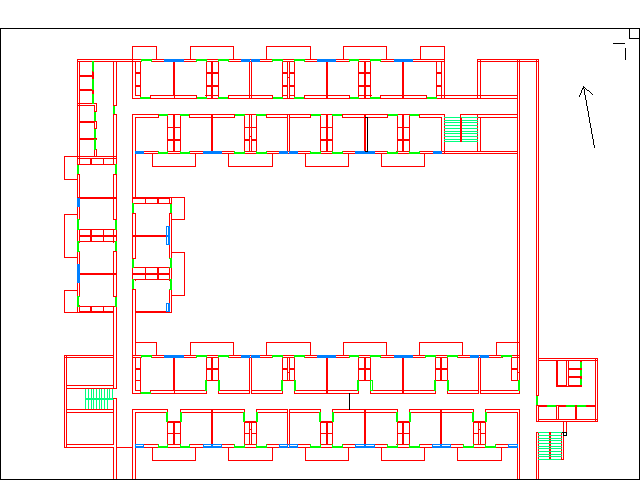
\includegraphics[width=6in]{figures/ravindra_map.png}
    \caption{A map of the experimental environment\label{fig:ravindra_map}}
\end{figure}


\section{Simple Dead Reckoning}

As discussed in the Literature Review (Chapter \ref{chap:literature_review}) and
in the Proposed Work (Chapter \ref{chap:proposed_method}), it is impossible to
directly obtain displacement information by double integration of the
accelerometer data. Hence, the step detection method was employed for tracking
the motion of the device as held by a walking human.

\subsection{Step detection procedure}

Step detection for dead reckoning was done using accelerometer sensor data.
Two different methods were employed and the simple zero crossing method on 
unfiltered data was used as control to estimate the increase in accuracy of the
step detection procedure. A simple clamping technique was employed to filter the
raw acceleration as described in Section \ref{sec:NoiseClamping}.

The effect of the clamping on the raw accelerometer data is shown in 
Figure \ref{fig:accel_raw}. Figure \ref{fig:accel_diff} shows the sensor noise
that is rejected around zero enabling clean detection of peaks corresponding to
the steps.

The comparative graph of the performance of the step detection procedures 
is shown in Figure \ref{fig:csteps}. The correspondence to the ground truth
is shown in Table \ref{tbl:step_table}.

\begin{table}[tbph]
\centering
\begin{tabular}{||l|c||}
\hline
\hline
\textbf{Algorithm} & \textbf{Steps Detected} \\
\hline

Simple Zero Crossings Count & 109 \\
Zero Crossings on Filtered Data & 41 \\
Peaks and Valley Method & 41 \\
\textbf{Ground Truth} & \textbf{40} \\
\hline
\hline
\end{tabular}
\caption{Step Detection Performance\label{tbl:step_table}}
\end{table}

It can be seen that a simple Zero Crossing method performs similarly to the 
Peaks and Valley method. From the time based graph plotted in 
Figure \ref{fig:csteps}, it can be seen that the Peaks and Valley method 
slightly lags the Zero Crossing method in time. This is to be expected as this
method detects a step only when the next peak is detected and thus suffers a 
lag of about half a step.

\begin{figure}[tbph]
    \centering
    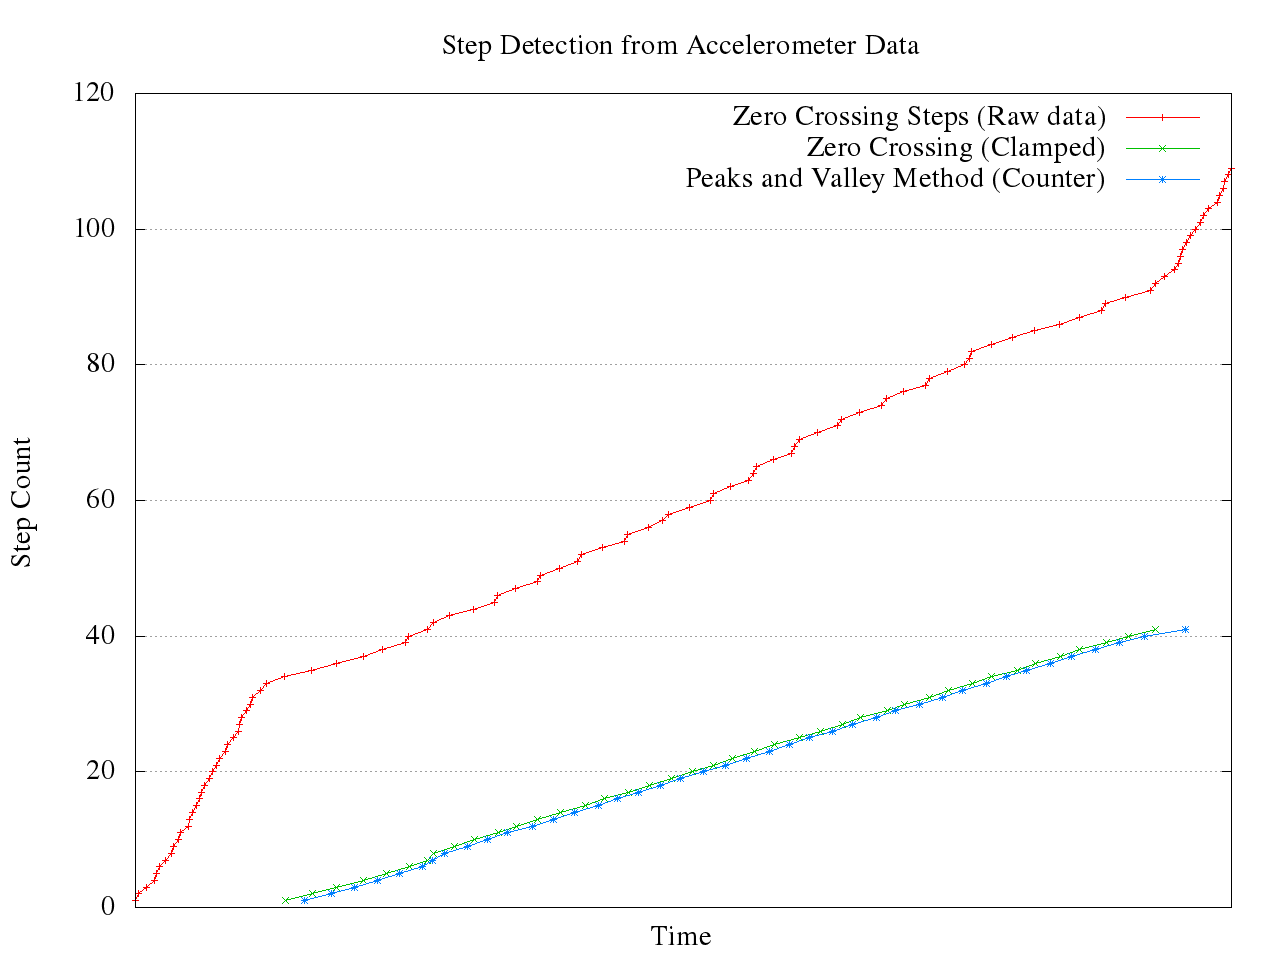
\includegraphics{figures/csteps.png}
    \caption{Performance of Step Detection Algorithms\label{fig:csteps}}
\end{figure}

\begin{figure}[tbph]
    \centering
    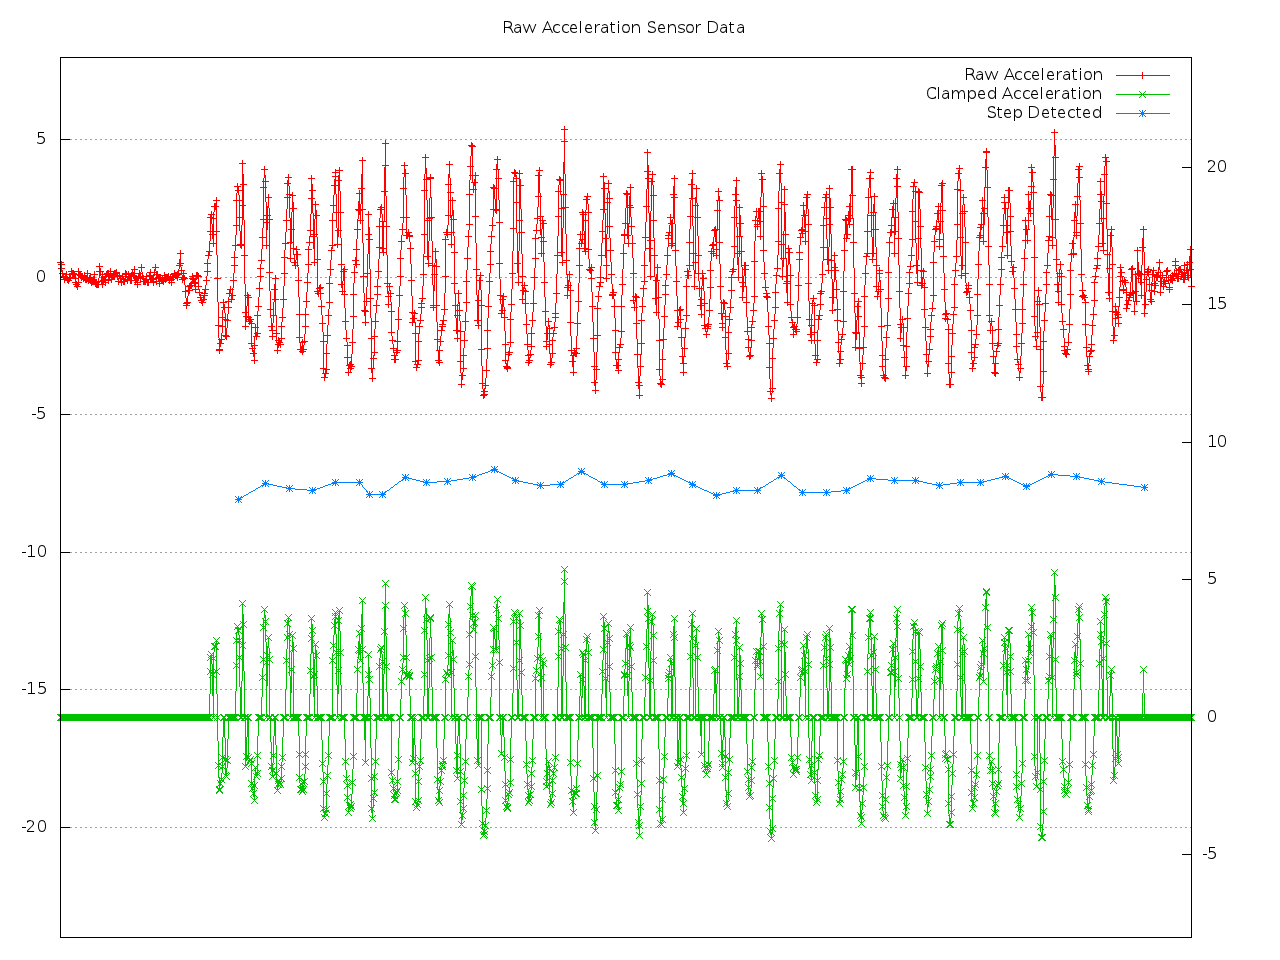
\includegraphics{figures/accel_raw.png}
    \caption{Performance of the Filtering algorithm \label{fig:accel_raw}}
\end{figure}

\begin{figure}[tbph]
    \centering
    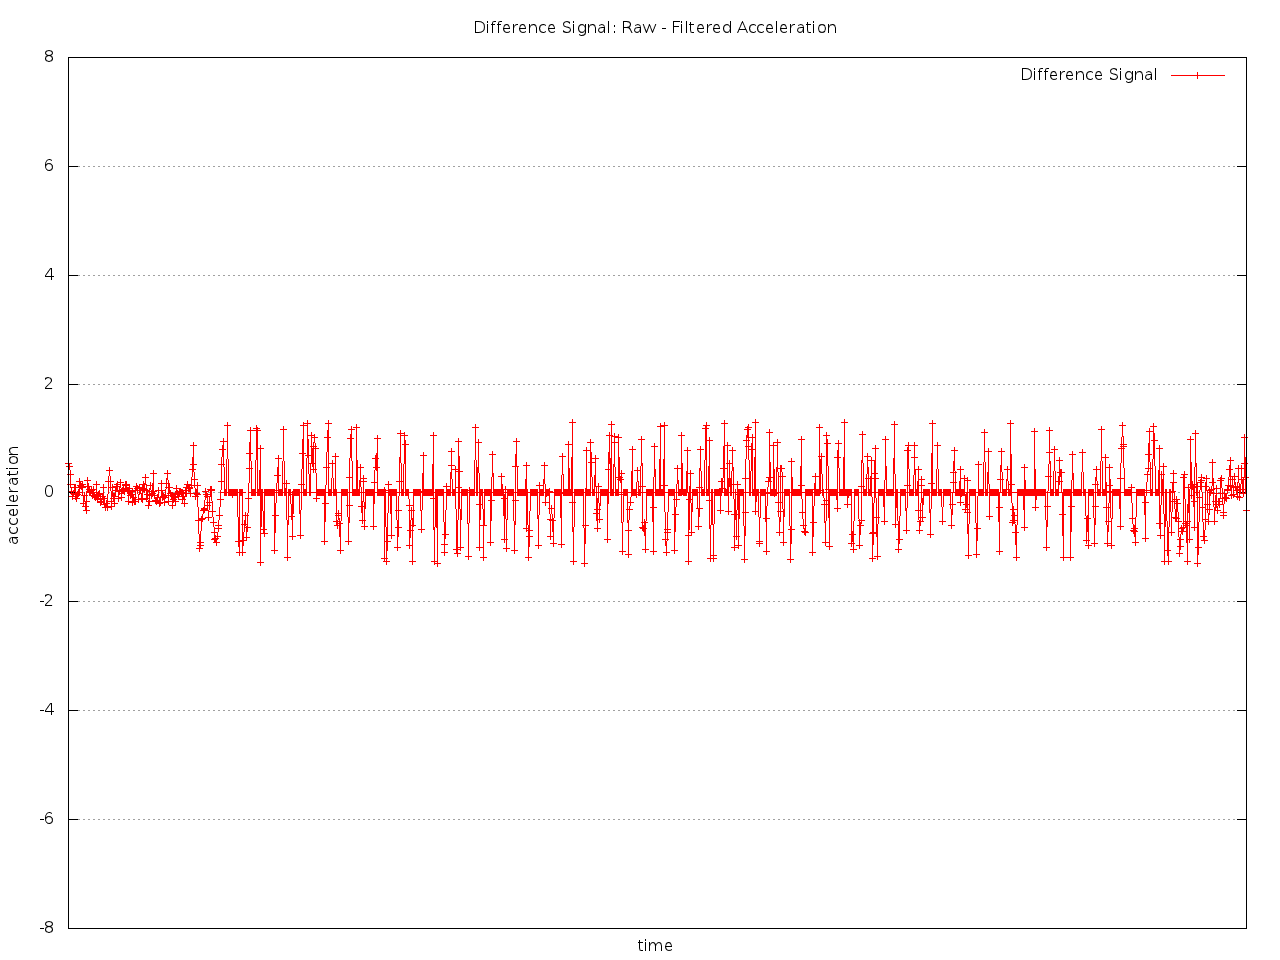
\includegraphics{figures/accel_diff.png}
    \caption{Rejected signal from the Accelerometer sensor \label{fig:accel_diff}}
\end{figure}


\subsection{First Fix}

For any dead reckoning algorithm, it is important to provide a good starting
point. Low error in the starting location contributes to better
tracking performance.

In order to provide the starting point to the algorithm two approaches were
implemented:

\begin{enumerate}
\item Directly choose the starting location on a map using the capacitive 
    touchscreen
\item Select the starting location based on QRCode recognition using the onboard
    camera. The QRCodes were printed and pasted at specific locations 
    in the area under test.
\end{enumerate}

Five test subjects were asked to mark out their current position on a
map by simply touching the corresponding location on the map shown on the 
touchscreen of the device. The map was shown at a fixed resolution to all 
test subjects in order to make their responses comparable. 

The test were also allowed to retry locating themselves on the map in case they
were not satisfied with their initial results. All their location attempts were
logged for later analysis. The results are summarized in 

\subsubsection{Direct Location on a Map}

\subsubsection{Camera based QRCode Method}
QRCode acquisition was successful at distances ranging from 30 cm to 1 m using
the Android phone. 

\subsection{Determining the Training Constant}

\section{Plain Wifi Based Positioning}
\subsection{Case 1: Dead reckoning with NN wifi positioning}
\subsection{Case 2: Dead reckoning with KNN averaging}
\subsection{Case 3: Dead reckoning with clamped wifi positioning}

\section{Particle Filter Performance}
\subsection{Case 1: Probability of crossing walls is 0}
\subsection{Case 2: Probability of crossing walls is finite}
\subsection{Case 3: Resampling of impoverished data points with duplication}
\subsection{Case 4: Resampling with introduction of Gaussian noise}
\subsection{Case 4a: Use of averaged data points v/s random weighted data point}
\subsection{Case 5: Accounting for bias in orientation sensor}
\subsection{Case 6: Accounting for step size bias.}
\subsection{Case 7: Simple post processing of output.??}
\subsection{Case 8: Simple heuristics to deal with impoverished samples}
(retry, retry with greater inaccuracy)

\section{Particle filter + Wifi data}
TODO

\subsection{Case 1: Use of Wifi data for accounting for drift errors}
\subsection{Case 2: Use of Oriented Wifi data for accounting for drift errors}
\subsection{Case 3: Use of clamped wifi data for accounting for drift errors}
\subsection{Case 4: Use of area Restricted Wifi data for accounting for drift errors}

\section{Signal Strength Map}

TODO if time permits
Wifi signal strength map developed using crowdsourced data for use in systems such as RedPin.

\section{Issues faced}
Incorrect step sizes yielded states in which no further progress was possible using data from the inertial sensors. Hence we had to resort to wifi data to get out of the blind spot.

Limited processing power and near-realtime time constraints of operation constrain computational 
complexity of the solution.

Surveying is the biggest issue in this system.

